\lstset{%
    language={C},%
    emph={APPROX, PRECISE, ENDORSE},%
}

\newcommand{\sysname}{ACCEPT\xspace}
\newcommand{\term}[1]{\emph{#1}}
\newcommand{\annpermit}{\lil{ACCEPT_PERMIT}\xspace}
\newcommand{\annforbid}{\lil{ACCEPT_FORBID}\xspace}

% Shifting terminology.
\newcommand{\precisepure}{approximatable\xspace}
\newcommand{\precisepurity}{approximatability\xspace}
\newcommand{\Precisepurity}{Approximatability\xspace}

% References.
\renewcommand{\secref}[1]{Section~\ref{accept:#1}}
\newcommand{\Sref}[1]{Section~\ref{accept:#1}}
\renewcommand{\figref}[1]{Figure~\ref{accept:#1}}
\renewcommand{\tabref}[1]{Table~\ref{accept:#1}}

% Generated results values.
\edef\result#1{%
\ifstrequal{#1}{fft-mlc-cycles}{2.68}{}%
\ifstrequal{#1}{fft-mlc-error}{1\%}{}%
\ifstrequal{#1}{fft-mlc-speedup}{1.13$\times$}{}%
\ifstrequal{#1}{fft-mlc-stripe-cycles}{2.44}{}%
\ifstrequal{#1}{fft-mlc-stripe-error}{4\%}{}%
\ifstrequal{#1}{fft-mlc-stripe-speedup}{1.24$\times$}{}%
\ifstrequal{#1}{image-mlc-cycles}{1.41}{}%
\ifstrequal{#1}{image-mlc-error}{1\%}{}%
\ifstrequal{#1}{image-mlc-flash-cycles}{13.0}{}%
\ifstrequal{#1}{image-mlc-flash-error}{9\%}{}%
\ifstrequal{#1}{image-mlc-flash-speedup}{1.6$\times$}{}%
\ifstrequal{#1}{image-mlc-speedup}{2.14$\times$}{}%
\ifstrequal{#1}{image-mlc-stripe-cycles}{1.41}{}%
\ifstrequal{#1}{image-mlc-stripe-error}{1\%}{}%
\ifstrequal{#1}{image-mlc-stripe-speedup}{2.14$\times$}{}%
\ifstrequal{#1}{jmeint-mlc-cycles}{1.87}{}%
\ifstrequal{#1}{jmeint-mlc-error}{2\%}{}%
\ifstrequal{#1}{jmeint-mlc-speedup}{1.62$\times$}{}%
\ifstrequal{#1}{jmeint-mlc-stripe-cycles}{1.71}{}%
\ifstrequal{#1}{jmeint-mlc-stripe-error}{10\%}{}%
\ifstrequal{#1}{jmeint-mlc-stripe-speedup}{1.77$\times$}{}%
\ifstrequal{#1}{lu-mlc-cycles}{1.98}{}%
\ifstrequal{#1}{lu-mlc-error}{6\%}{}%
\ifstrequal{#1}{lu-mlc-speedup}{1.53$\times$}{}%
\ifstrequal{#1}{lu-mlc-stripe-cycles}{1.98}{}%
\ifstrequal{#1}{lu-mlc-stripe-error}{5\%}{}%
\ifstrequal{#1}{lu-mlc-stripe-speedup}{1.53$\times$}{}%
\ifstrequal{#1}{mc-mlc-cycles}{1.71}{}%
\ifstrequal{#1}{mc-mlc-error}{4\%}{}%
\ifstrequal{#1}{mc-mlc-speedup}{1.77$\times$}{}%
\ifstrequal{#1}{mc-mlc-stripe-cycles}{1.59}{}%
\ifstrequal{#1}{mc-mlc-stripe-error}{10\%}{}%
\ifstrequal{#1}{mc-mlc-stripe-speedup}{1.91$\times$}{}%
\ifstrequal{#1}{ml-mlc-cycles}{1.71}{}%
\ifstrequal{#1}{ml-mlc-error}{6\%}{}%
\ifstrequal{#1}{ml-mlc-flash-cycles}{19.7}{}%
\ifstrequal{#1}{ml-mlc-flash-error}{8\%}{}%
\ifstrequal{#1}{ml-mlc-flash-speedup}{1.05$\times$}{}%
\ifstrequal{#1}{ml-mlc-speedup}{1.77$\times$}{}%
\ifstrequal{#1}{ml-mlc-stripe-cycles}{1.41}{}%
\ifstrequal{#1}{ml-mlc-stripe-error}{0\%}{}%
\ifstrequal{#1}{ml-mlc-stripe-speedup}{2.14$\times$}{}%
\ifstrequal{#1}{mlc-flash-mean-cycles}{16.4}{}%
\ifstrequal{#1}{mlc-flash-mean-speedup}{1.26$\times$}{}%
\ifstrequal{#1}{mlc-mean-cycles}{1.91}{}%
\ifstrequal{#1}{mlc-mean-speedup}{1.59$\times$}{}%
\ifstrequal{#1}{mlc-stripe-mean-cycles}{1.79}{}%
\ifstrequal{#1}{mlc-stripe-mean-speedup}{1.7$\times$}{}%
\ifstrequal{#1}{nn-mlc-cycles}{1.87}{}%
\ifstrequal{#1}{nn-mlc-error}{1\%}{}%
\ifstrequal{#1}{nn-mlc-flash-cycles}{16.5}{}%
\ifstrequal{#1}{nn-mlc-flash-error}{10\%}{}%
\ifstrequal{#1}{nn-mlc-flash-speedup}{1.26$\times$}{}%
\ifstrequal{#1}{nn-mlc-speedup}{1.62$\times$}{}%
\ifstrequal{#1}{nn-mlc-stripe-cycles}{1.71}{}%
\ifstrequal{#1}{nn-mlc-stripe-error}{1\%}{}%
\ifstrequal{#1}{nn-mlc-stripe-speedup}{1.77$\times$}{}%
\ifstrequal{#1}{pa-mlc-cycles}{1.71}{}%
\ifstrequal{#1}{pa-mlc-error}{3\%}{}%
\ifstrequal{#1}{pa-mlc-flash-cycles}{16.5}{}%
\ifstrequal{#1}{pa-mlc-flash-error}{6\%}{}%
\ifstrequal{#1}{pa-mlc-flash-speedup}{1.26$\times$}{}%
\ifstrequal{#1}{pa-mlc-speedup}{1.77$\times$}{}%
\ifstrequal{#1}{pa-mlc-stripe-cycles}{1.59}{}%
\ifstrequal{#1}{pa-mlc-stripe-error}{5\%}{}%
\ifstrequal{#1}{pa-mlc-stripe-speedup}{1.91$\times$}{}%
\ifstrequal{#1}{raytracer-mlc-cycles}{1.59}{}%
\ifstrequal{#1}{raytracer-mlc-error}{7\%}{}%
\ifstrequal{#1}{raytracer-mlc-speedup}{1.91$\times$}{}%
\ifstrequal{#1}{raytracer-mlc-stripe-cycles}{1.59}{}%
\ifstrequal{#1}{raytracer-mlc-stripe-error}{6\%}{}%
\ifstrequal{#1}{raytracer-mlc-stripe-speedup}{1.91$\times$}{}%
\ifstrequal{#1}{recycle-fft-qos-ext}{5\%}{}%
\ifstrequal{#1}{recycle-fft-total-ext}{34\%}{}%
\ifstrequal{#1}{recycle-image-ext}{90\%}{}%
\ifstrequal{#1}{recycle-jmeint-qos-ext}{25\%}{}%
\ifstrequal{#1}{recycle-jmeint-total-ext}{34\%}{}%
\ifstrequal{#1}{recycle-lu-qos-ext}{11\%}{}%
\ifstrequal{#1}{recycle-lu-total-ext}{32\%}{}%
\ifstrequal{#1}{recycle-mc-qos-ext}{32\%}{}%
\ifstrequal{#1}{recycle-mc-total-ext}{34\%}{}%
\ifstrequal{#1}{recycle-mean-all-ext}{23\%}{}%
\ifstrequal{#1}{recycle-mean-nv-ext}{36\%}{}%
\ifstrequal{#1}{recycle-mean-qos-ext}{18\%}{}%
\ifstrequal{#1}{recycle-mean-total-ext}{34\%}{}%
\ifstrequal{#1}{recycle-ml-ext}{17\%}{}%
\ifstrequal{#1}{recycle-nn-ext}{17\%}{}%
\ifstrequal{#1}{recycle-pa-ext}{42\%}{}%
\ifstrequal{#1}{recycle-raytracer-qos-ext}{39\%}{}%
\ifstrequal{#1}{recycle-raytracer-total-ext}{39\%}{}%
\ifstrequal{#1}{recycle-smm-qos-ext}{20\%}{}%
\ifstrequal{#1}{recycle-smm-total-ext}{29\%}{}%
\ifstrequal{#1}{recycle-sor-qos-ext}{20\%}{}%
\ifstrequal{#1}{recycle-sor-total-ext}{32\%}{}%
\ifstrequal{#1}{recycle-zxing-qos-ext}{2\%}{}%
\ifstrequal{#1}{recycle-zxing-total-ext}{37\%}{}%
\ifstrequal{#1}{smm-mlc-cycles}{1.87}{}%
\ifstrequal{#1}{smm-mlc-error}{3\%}{}%
\ifstrequal{#1}{smm-mlc-speedup}{1.62$\times$}{}%
\ifstrequal{#1}{smm-mlc-stripe-cycles}{1.87}{}%
\ifstrequal{#1}{smm-mlc-stripe-error}{2\%}{}%
\ifstrequal{#1}{smm-mlc-stripe-speedup}{1.62$\times$}{}%
\ifstrequal{#1}{sor-mlc-cycles}{2.25}{}%
\ifstrequal{#1}{sor-mlc-error}{3\%}{}%
\ifstrequal{#1}{sor-mlc-speedup}{1.35$\times$}{}%
\ifstrequal{#1}{sor-mlc-stripe-cycles}{2.1}{}%
\ifstrequal{#1}{sor-mlc-stripe-error}{7\%}{}%
\ifstrequal{#1}{sor-mlc-stripe-speedup}{1.44$\times$}{}%
\ifstrequal{#1}{zxing-mlc-cycles}{2.25}{}%
\ifstrequal{#1}{zxing-mlc-error}{4\%}{}%
\ifstrequal{#1}{zxing-mlc-speedup}{1.35$\times$}{}%
\ifstrequal{#1}{zxing-mlc-stripe-cycles}{2.1}{}%
\ifstrequal{#1}{zxing-mlc-stripe-error}{9\%}{}%
\ifstrequal{#1}{zxing-mlc-stripe-speedup}{1.44$\times$}{}%
}


\begin{figure}[t]
\centering
\makebox[\textwidth][c]{%
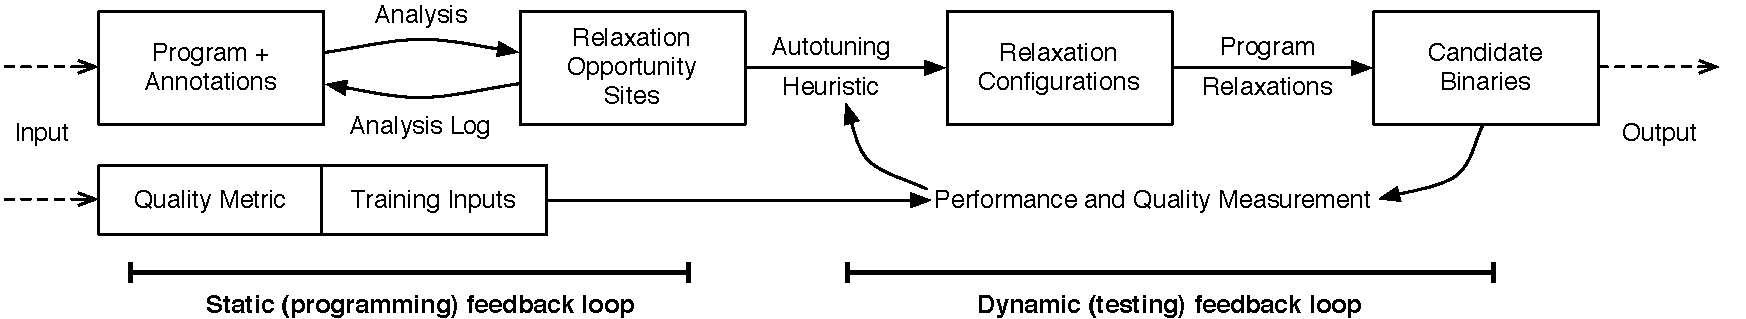
\includegraphics[width=1.3\textwidth]{figs/overview.pdf}%
}
\caption{Overview of the \sysname compiler workflow.}
\label{accept:fig:overview}
\end{figure}

\section{Introduction}\label{accept:sec:intro}

Approximate computing includes a diverse spectrum of
implementation techniques, spanning both hardware and software:
everything from adjusting numerical representations
to exploiting analog circuits.
Some work relies on programmers for manual reasoning to control
approximation's
potential effects~\cite{npu, flikker, races-ibm, perforation},
while other work proposes automated transformation based on code
patterns or exhaustive search~\cite{green, paraprox, sage}.
Manual code editing can be tedious and error-prone, especially since
important safety invariants are at stake.
Conversely, full automation eliminates a crucial element of
visibility and control.
Programmers must trust the automated system; they have no recourse when
opportunities are missed or invariants are broken.

This chapter describes \sysname
(an Approximate C Compiler for Energy and Performance Trade-offs),
a framework for approximation that balances automation with programmer
guidance.
\sysname is \emph{controlled} because it preserves programmer intention
expressed via code annotations.
A static analysis rules out
unintended side effects. The programmer participates in a feedback loop with
the analysis to enable more approximation
opportunities.
\sysname is \emph{practical} because it facilitates a range
of approximation techniques that work on currently available hardware.
Just as a traditional compiler framework provides common tools to support
optimizations,
\sysname's building blocks help implement automatic
approximate transformations based on programmer guidance and dynamic feedback.

\sysname's architecture combines static and dynamic components.
The frontend, built atop LLVM~\cite{llvm}, extends the syntax of C and C++ to
incorporate an \lil{APPROX} keyword that programmers use to annotate types, as
in \chref{enerj}.
\sysname's central analysis, \emph{\precisepurity}, identifies coarse-grained
regions of code that can
affect only approximate values.
Coarse region selection is crucial for safe approximation strategies:
client optimizations use the results to
transform code and offload to accelerators while preserving static safety
properties.
After compilation, an autotuning component measures program executions
and uses heuristics to identify program variants that maximize performance and output quality.
To incorporate application insight, \sysname furnishes programmers with feedback
to guide them toward better annotations.


\sysname is an end-to-end framework that makes existing proposals for approximate
program transformations practical and disciplined.
Its contributions are:
\begin{itemize}
\item A programming model for program relaxation that combines lightweight
annotations with compiler analysis feedback
to guide programmers toward effective relaxations;

\item An autotuning system that efficiently searches for a program's
best approximation parameters;

\item A core analysis library that identifies code that can be safely relaxed
or offloaded to an approximate accelerator;

\item A prototype implementation demonstrating both pure-software optimizations
and hardware acceleration using an off-the-shelf FPGA part.
\end{itemize}

\noindent
We evaluate \sysname across three platforms:
a standard Intel-based server;
a mobile SoC with an on-chip FPGA, which we use as an approximate accelerator;
and an ultra-low-power, energy-harvesting embedded microcontroller where
performance is critical to applications' viability.
The experiments demonstrate average speedups of \result{speedup-x86-mean},
\result{speedup-zynq-mean}, and \result{speedup-msp430-mean} on the
three platforms, respectively,
with quality loss under 10\%.

We also report qualitatively on the programming experience.
Novice C++ programmers were able to apply \sysname to
legacy software to obtain new speedups.
\sysname's combination of static analysis and dynamic measurement alleviates
much of the manual labor from the process of applying
approximation without sacrificing transparency or control.

The \sysname framework is open source and ready for use as research
infrastructure.
It provides the necessary language and compiler support to prototype and
evaluate new strategies for approximation,
reducing the need to reinvent these components for each new research
evaluation.


\section{Introduction}
\label{sec:intro}

Accuracy and reliability are fundamental tenets in computer system design.
Programmers can expect that the processor never exposes timing
errors, and networking stacks typically aim to provide reliable transports
even on unreliable physical media.
When errors do occasionally happen, we treat them as exceptional outliers, not
as part of the system abstraction.
Cosmic rays can silently flip bits in DRAM, for example,
but the machine will typically use error-correcting codes to
maintain the illusion for programmers that the memory is infinitely reliable.

But abstractions with perfect accuracy come at a cost.
Chips need to choose conservative clock rates to banish timing errors,
storage and communication channels incur error-correction overhead,
and parallelism requires expensive synchronization.

Meanwhile, many applications have intrinsic tolerance to inaccuracy.
Applications in domains like computer vision, media
processing, machine learning, and sensor data analysis already incorporate
imprecision into their design.
Large-scale data analytics focus on aggregate trends rather than the integrity
of individual data elements.
In domains such as computer vision and robotics, there are no perfect answers:
results can vary in their usefulness, and the output quality is always in
tension with the resources that the software needs to produce them.
All these applications are \emph{approximate
programs}: a range of possible values can be considered ``correct'' outputs
for a given input.

From the perspective of an approximate program, today's
systems are overprovisioned with accuracy. Since the program is resilient, it
does
not need every arithmetic operation to be precisely correct and every bit of
memory to be preserved at the same level of reliability.
\emph{Approximate computing} is a research agenda that seeks to better match
the accuracy in system abstractions with the needs of approximate
programs.


\paragraph{Disciplined approximation}

The central challenge in approximate computing is forging abstractions that
make imprecision \emph{controlled and predictable} without sacrificing its
efficiency benefits.
This goal of this dissertation is to design hardware and software around
approximation-aware abstractions that, together, make accuracy--efficiency
trade-offs attainable for programmers.
My work examines approximate abstractions
in the contexts of programming languages, computer architecture,
memory technologies, compilers, and software development
tools.

\section{Research Principles}

The work in this dissertation is organized around five principles
for the design of disciplined approximate abstractions.
These themes represent the collective findings of the concrete research
projects described later.
The principles are:
%
\begin{enumerate}
\item Result quality is an application-specific property.
\item Approximate abstractions should distinguish between safety properties
    and quality properties.
\item Hardware and software need to collaborate to reach the best
    potential of approximate computing.
\item Approximate programming models need to incorporate probability and
    statistics.
\item The granularity of approximation represents a trade-off between
    generality and potential efficiency.
\end{enumerate}
%
This section outlines each finding in more detail.

\subsection{Result Quality is Application Specific}
\label{sec:princ:appspecific}

Since approximate computing navigates trade-offs between efficiency and result
quality, it needs definitions of both sides of the balance.
While \emph{efficiency} can have universal definitions---the time to
completion, for example, or the number of joules consumed---output
\emph{quality} is more subtle.
A key tenet in this work is is that applications must define ``output
quality'' case by case:
the platform cannot define quality without information from the programmer.

Following this philosophy, the system designs in this dissertation assume that
each approximate program comes with a \emph{quality metric}, expressed as
executable code, that scores the program's output on a continuous scale from
0.0 to 1.0.
A quality metric is the approximate-computing analog to a traditional software
\emph{specification}, which typically makes a binary decision about whether an
implementation is correct or incorrect.
Just as ordinary verification and optimization tools start from a
specification, approximate-computing tools start with a quality metric.

\subsection{Safety vs.~Quality}
\label{sec:princ:safety}

At first glance, a quality metric seems like sufficient information to specify
an application's constraints on approximation.
If the system can guarantee that a program's output will always have a quality
score above $q$, and the programmer decides that $q$ is good enough, what
could possibly go wrong?

In reality, it can be difficult or impossible for systems to prove arbitrary
quality bounds with perfect certainty.
Realistic tools can often only certify, for example, that any output's quality
score will be at least $q$ \emph{with high probability},
or that \emph{nearly every output} will exceed quality $q$ but rare edge cases
may do worse.
Even more fundamentally, it can be difficult for programmers to devise formal
quality metrics that capture every possible factor in their intuitive notion
of output quality.
Quality metrics can be simpler if their scope is narrowed to data where they
are most relevant: the pixels in an output image, for example, but not the
header data.

To that end, this dissertation embraces \emph{safety} as a separate concept
from quality.
A safety property, in the context of approximate computing, is a guarantee
that part of a program \emph{never} deviates from its precise counterpart---in
other words, that it matches the semantics of a traditional, non-approximate
system.
A quality property, in contrast, constrains the \emph{amount} that approximate
program components deviate from their precise counterparts.

In practice, we find a first-order distinction between \emph{no approximation at
all} and \emph{approximation of some nonzero degree} both simplifies reasoning
for programmers and makes tools more tractable.
My work has demonstrated that the two kinds of properties can be amenable to
very different techniques:
information flow tracking (\chref{enerj}) is appropriate for safety, for
example, but statistical hypothesis testing (\chref{passert}) is better for
quality.

\subsection{Hardware--Software Co-Design}

% Approximate computing techniques cover a broad range of approaches,
% from hardware to software.
Some of the most promising ideas unlock new sources of efficiency that are
only available in hardware:
exploiting the analog behavior of transistors, for example,
or mitigating the cost of error correction in memory modules.
Because approximation techniques have subtle and wide-ranging effects on
program behavior, however,
designs that apply them \emph{obliviously} are unworkable.
Instead, researchers should co-design hardware techniques with their software
abstractions to ensure that programmers can control imprecision.

Hardware designs can also rely on guarantees from software---the language or
compiler---to avoid unnecessary complexity.
The Truffle approximate CPU~\cite{truffle}, for example, avoids expensive
hardware consistency checks by exploiting EnerJ's compile-time enforcement of
type safety.
Wherever possible, hardware researchers should offload responsibilities to
complementary software systems.

\subsection{Programming with Probabilistic Reasoning}

Often, the most natural ways to reason about approximation and quality use
probabilistic tools.
Probabilistic reasoning lets us show show statements such as \emph{this output
will be high-quality with at least probability $P$} or \emph{an input randomly
selected from this distribution leads to a high-quality output with
probability $P'$}.
These probabilistic statements can simultaneously match the nondeterministic behavior
of approximate systems~\cite{truffle, npu, approxstorage}
and correspond to software quality criteria~\cite{decaf, passert}.

To support reasoning about quality, approximate
programming models need to incorporate abstractions for statistical behavior.
The DECAF type system, in \chref{decaf}, and
probabilistic assertions, in \chref{passert}, represent two
complementary approaches to reasoning about probabilistic quality
properties.

These approaches dovetail with the recent expansion of interest in
\emph{probabilistic programming languages}, which seek to augment
machine-learning techniques with language abstractions~\cite{church}.
Approximate programming systems can adapt lessons from this body of research.

\subsection{Granularity of Approximation}
\label{sec:princ:granularity}

The \emph{granularity} at which approximate computing applies is a
nonintuitive but essential factor in its success.
My and other researchers' work has explored approximation strategies at
granularities of both extremes:
fine-grained approximations that apply to individual instructions and
individual words of memory (e.g., Truffle~\cite{truffle});
and coarse-grained approximations that holistically transform entire
algorithms (e.g., neural acceleration~\cite{npu}).

A technique's granularity affects its
generality and its efficiency potential.
A fine-grained approximation can be very general:
an approximate multiplier unit, for example, can potentially apply to any
multiplication in a program.
But the efficiency gains are fundamentally limited to \emph{non-control} components,
since control errors can disrupt execution arbitrarily.
Even if an approximate multiplier unit can be very efficient,
the same technique can never
improve the efficiency of a branch, an address calculation,
or even the
scheduling of an approximate multiply instruction.
Approximations that work at a coarser granularity can address control costs,
so their potential gains are larger.
But these techniques tend to apply more narrowly:
techniques that pattern-match on algorithm structures~\cite{paraprox},
for example, place nuanced restrictions on the code they can transform.

The EnerJ language in \chref{enerj} was initially designed for
fine-grained hardware approximation techniques such as low-voltage functional
units.
While the granularity was good for programmability, it was bad for efficiency:
our detailed hardware design for fine-grained hardware
approximation~\cite{truffle} demonstrated limited benefit.
The ACCEPT compiler in \chref{accept} bridges the gap: its analysis
library and optimizations exploit the fine-grained annotations from EnerJ to
safely apply coarse-grained optimizations.


\section{Abstractions for Disciplined Approximation}

This dissertation supports the above research principles using a set of
concrete system designs.
The systems comprise programming-language constructs that express
applications' resilience to approximation along with system-level
techniques for exploiting that latent resilience to gain efficiency.
This section serves as an overview of the interlocking designs;
Parts~\ref{part:programming} and~\ref{part:systems} give the full details.

\subsection{Controlling Safety and Quality}

The first set of projects consists of language abstractions that give
programmers control over safety and quality in approximate programs.

\subsubsection{Information Flow Tracking for General Safety}

EnerJ, described in \chref{enerj}, is a type system for enforcing safety in
the presence of approximation.
The key insight in EnerJ is that approximate programs tend to consist of two
intermixed kinds of storage and computation:
critical control components
and non-critical data components.
The latter, which typically form the majority of the program's execution,
are good candidates for approximation,
while the former should be protected from error and carry traditional
semantics.

EnerJ lets programmers enforce a separation between critical and non-critical
components.
It uses a type system that
borrows from static information
flow systems for security~\cite{jif, infflow-survey} to provide a static
noninterference guarantee for precise data.
EnerJ extends Java with two type qualifiers, \code{@Approx} and
\code{@Precise}, and uses a subtyping relationship to prevent
approximate-to-precise information flow.
Using EnerJ, programmers can rely
on a proof that data marked as precise remains untainted by the errors arising
from approximation.

A key design goal in EnerJ is its \emph{generality:}
the language aims to encapsulate a range of approximation strategies under a
single abstraction.
Its type system covers approximate storage via the types of variables and
fields;
approximate processor logic via overloading of arithmetic operators;
and even user-defined approximate algorithms using dynamic method dispatch
based on its approximating qualifiers.

EnerJ addresses safety, not quality:
a variable with the type \code{@Approx float} can be arbitrarily incorrect and
EnerJ does not seek to bound its incorrectness.
By leaving the complementary concern of controlling quality to separate
mechanisms, EnerJ keeps its type system simple.

\subsubsection{Extending EnerJ with Probability Types}

DECAF, in \chref{decaf}, extends EnerJ's type-based approach to safety with
quality guarantees.
The idea is to generalize the original \code{@Approx} type qualifier to a
parameterized qualifier \code{@Approx($p$)}, where $p$ dictates the
\emph{degree} of approximation.
Specifically, in DECAF, $p$ is the lower bound on the probability that a value
is \emph{correct:} that the value in an approximate execution equals its
counterpart in a completely precise execution of the same program.
DECAF defines sound type rules for introducing and propagating these
correctness probabilities.

DECAF's added sophistication over EnerJ's simple two-level system comes at a
cost in complexity:
a type system that requires probability annotations on every expression
would quickly become infeasible for programmers.
To mitigate annotation overhead, DECAF adds type inference.
Sparse probability annotations on the inputs and outputs of coarse-grained
subcomputations are typically enough for DECAF's inference system to determine
the less-intuitive probabilities for intermediate values.
Crucially, DECAF places no constraints on where programmers can write explicit
annotations:
developers can write probabilities where they make the most sense and leave
the remaining details to the compiler.

DECAF addresses the limitations of a conservative quality analysis using
an optional dynamic-tracking mechanism.
The inference system also allows efficient code reuse by specializing
functions according to the accuracy constraints of their calling contexts.

\subsubsection{Probabilistic Assertions}

DECAF's approach to controlling quality achieves strong probabilistic
guarantees by constraining the range of possible approximation strategies:
it works only with techniques where errors appear at an operation granularity;
whey they occur randomly but rarely; and when the error probability is
independent of the input values.

A complementary project takes the opposite approach:
it accommodates any probability distribution, but it offers weaker
guarantees.
The idea is to use statistical hypothesis tests to prove properties up to a
\emph{confidence level:}
to allow a small probability of ``verifying'' a false property.

The technique is based on a new language construct called a
\emph{probabilistic assertion}.
The construct is analogous to a traditional assertion: \code{assert $e$}
expresses that the expression $e$ must always be true.
A probabilistic assertion:
%
\begin{lstlisting}
passert $e$, $p$, $c$
\end{lstlisting}
%
indicates that $e$ must
be true with at least probability $p$, and the system has to prove the
property at confidence level $c$.
These assertions can encode important quality properties in approximate
programs, such as bounds on the frequency of ``bad'' pixels produced by an
image renderer.
The same construct is useful in other domains where probabilistic behavior is
essential, such as when dealing with noisy sensors.

\chref{passert} describes probabilistic assertions in more detail
along with a workflow for verifying them efficiently.
The verifier uses a symbolic-execution technique to extract a representation
of a program's probabilistic behavior: a Bayesian network.
The verifier can optimize this Bayesian-network representation using
off-the-shelf statistical properties that are difficult to apply to the
original program code.
The complete workflow can make probabilistic-assertion verification dozens of
times faster to check than a naive stress-testing approach.

\subsection{Exploiting Resilience for Efficiency}

The second category of research is on the implementation of systems that
exploit programs' tolerance for approximation to improve efficiency.
This dissertation describes two projects: an architectural technique and an
end-to-end compiler toolchain.
A primary concern in both systems is exposing an abstraction that fits with
the safety and quality constraints introduced in the above language
abstractions.

\subsubsection{Approximate Storage for Solid-State Memory Technologies}

One system design, detailed in \chref{approxstorage}, builds on a trend in hardware technologies.
It exploits unique properties of new solid-state memories,
such as flash memory and phase-change memory,
to implement two orthogonal trade-offs between resource and accuracy.

The first technique recognizes that the underlying material in these memory
technologies is analog.
Traditional designs build a clean digital abstraction on top of a
fundamentally analog memory cell.
Our technique addresses the cost of that digital abstraction by letting
applications opt into stochastic data retention.

The second technique embraces resistive memory technologies' tendency to wear
out.
Ordinarily, architectures need to detect failed memory blocks and avoid
storing data in them---limiting the memory module's useful lifetime.
Instead, in the context of an approximate application, we can harvest the otherwise-unusable
blocks and store approximate data in them.

Both strategies need a new set of common CPU and operating-system interfaces
to let software communicate error resilience and bit layout information.
We develop these abstractions to match the structure and semantics of EnerJ.

\subsubsection{ACCEPT: An Approximate Compiler}

The final system design takes a different tactic:
rather than simulating hypothetical hardware,
the idea is to build a practical infrastructure for experimenting with
approximation in the nearer term.
\chref{accept} introduces ACCEPT, an open-source compiler workflow designed both for
practitioners, to try out approximation techniques on their code,
and for researchers, to prototype and evaluate new ideas for approximation
strategies.

The first challenge that ACCEPT faces is to bridge the granularity gap (see
\secref{princ:granularity}, above).
EnerJ's fine-grained annotations can be more general and easier to apply to
programs,
but coarse-grained optimizations can offer better efficiency
gains---especially in the pure-software domain.
ACCEPT's interactive optimization architecture,
compiler analysis library,
and auto-tuner infrastructure help connect fine-grained safety annotations to
coarse-grained optimizations.

ACCEPT also addresses a second persistent challenge in approximate
programmability:
balancing automation with programmer control.
Fully manual approximation can be tedious and error prone,
but fully automatic systems can also frustrate developers by isolating them
from decisions that can break their code.
ACCEPT relies on the distinction between quality and safety (see
\secref{princ:safety}) to reconcile the extremes.
Type annotations resembling EnerJ's enforce safety, but programmers are kept
in the loop with an interactive optimization workflow to rule out unexpected
quality effects.
Together, the systems leverage the best of both factors:
programmer insight for preserving application-specific properties
and automatic compiler reasoning for identifying obscure data flows.

\section{Other Work}

The work in this document is intimately connected to other research I
collaborated on while at the University of Washington.
While this dissertation does not fully describe these related projects, their
influence is evident in the trajectory of projects that do appear here.
For context, this section describes a handful of other projects on approximate
hardware and developer tools.


\subsection{An Approximate CPU and ISA}

Truffle is a processor architecture that implements EnerJ's semantics to save
energy~\cite{truffle}. It uses a secondary, subcritical voltage that allows timing errors in
a portion of the logic and retention errors in a portion of the SRAM.

To expose the two voltages to software, we
designed an ISA extension that includes a notation of abstract approximation.
The code can choose dynamically to enable approximation
per instruction, per register, and per cache line.
A key challenge in the design was supporting an ISA that could efficiently
support an EnerJ-like programming model, where the precise and approximate
components of a program remain distinct but interleave at a fine grain.

Our simulation of the Truffle design space yielded results ranging from a 5\%
energy consumption \emph{increase} to a 43\% reduction.
These results emphasize the efficiency limits of very fine-grained
approximation (see the granularity principle in \secref{princ:granularity}).
Even in a maximally approximate program---in which every
arithmetic instruction and every byte of memory is marked as
approximate---much of Truffle's energy is spent on precise work. Fetching
code, scheduling instructions, indexing into SRAMs, computing addresses, and
tracking precision state all must be performed reliably.
Modern processors spend as much energy on
control as they do on computation itself, so any technique that optimizes only
computation will quickly encounter Amdahl's law.

The Truffle work in appears in the dissertation of Hadi
Esmaeilzadeh~\cite{hadi-thesis}.


\subsection{Neural Acceleration}
\label{sec:npu}

\emph{Neural acceleration} is a technique that explores the opposite end of
the granularity spectrum~\cite{npu, snnap}.
The idea is to use machine learning to imitate a portion of a computation by
observing its input--output behavior.
Then, we build a configurable hardware accelerator to efficiently execute the
learned model in place of the original code.
Our specific design uses neural networks:
since neural networks have
efficient hardware implementations, the transformed function can be much
faster and lower-power than the original code.

The coarse granularity pays off in efficiency: our simulations demonstrated a
3$\times$ average energy reduction.
But the coarser granularity comes at a cost of programmer visibility and
control.
Since the NPU technique treats the target code as a black box, the
programmer has no direct influence over the performance and accuracy of the
resulting neural network.
These conflicting objectives demonstrate the need for techniques that bridge
the granularity gap.

The original neural acceleration work also appears in Hadi Esmaeilzadeh's
dissertation~\cite{hadi-thesis}.
I also worked on a recent extension of the idea for programmable
logic~\cite{snnap}.


\subsection{Monitoring and Debugging Quality}

Many approaches to making approximation programmable focus on proving
conservative, static bounds.
As in traditional software development,
approximate computing also needs complementary dynamic techniques.
To this end, I contributed to a pair of techniques for dynamically controlling
result quality~\cite{approxdebug}.

The first dynamic system is a framework for monitoring quality in deployment.
The goal is to raise an exception whenever the program produces a ``bad''
output.
While the ideal monitoring system would directly measure the quality
degradation of every output,
perfect measurement is too expensive for run-time deployment.
Our framework provides a range of techniques for specific scenarios where we
can make monitoring cheap enough to be feasible.

The second system is a debugging tool.
The idea is that certain subcomputations can be more important to
quality than others, but that this difference is not necessarily obvious to
programmers.
The tool identifies and blames specific approximation decisions in a large
codebase when they are responsible for too much quality degradation.

The work on dynamic quality analysis appears in the dissertation of
Michael F.\ Ringenburg~\cite{ringenburg-thesis}.


\section{Organization}

The next chapter is a literature survey of work on efficiency--accuracy
trade-offs.
Historical context is particularly important to this dissertation because the
fundamental idea of exchanging accuracy for returns in efficiency is so old:
analog computers and floating-point numbers, for example, are prototypical
examples of
approximate-computing strategies.

Parts~\ref{part:programming} and~\ref{part:systems} form the core of the
dissertation.
They comprise five independent but interlocking research projects that
together build up abstractions for making approximate computing both tractable
and efficient.
%
Part~\ref{part:programming} describes three approaches to abstracting
approximation in programming languages:
EnerJ, a type system that uses type qualifiers to make approximation safe;
DECAF, an extension of EnerJ that adds probabilistic reasoning
about the likelihood that data is correct;
and probabilistic assertions, a strategy for efficiently verifying complex
probabilistic properties via sampling.
%
Part~\ref{part:systems} describes two system designs for implementing
efficiency--accuracy trade-offs:
a hardware architecture that exploits the nuances of resistive memory
technologies such as phase-change memory;
and an open-source compiler toolkit that provides the scaffolding to quickly
implement new approximation strategies while balancing programmability with
approximation's potential benefits.

Finally, \plurchref{conclusion} and~\ref{ch:future} look forward and
backward, respectively.
The retrospective chapter distills lessons from the work in this dissertation
about approximate computing and hardware--software co-design in general, and
the prospective chapter suggests next steps for bringing approximation into
the mainstream.

This dissertation also includes appendices that formalize the
programming-languages techniques in Part~\ref{part:programming} and prove
their associated theorems.


\section{Previously Published Material}

This dissertation comprises work published elsewhere in conference papers:
%
\begin{itemize}
\item \chref{enerj}:
\textit{EnerJ: Approximate Data Types for Safe and General Low-Power
Computation.}
Adrian Sampson, Werner Dietl, Emily Fortuna, Danushen Gnanapragasam, Luis Ceze, and Dan Grossman.
In Programming Language Design and Implementation (PLDI), 2011.
\cite{enerj}

\item \chref{decaf}:
\textit{Probability Type Inference for Flexible Approximate Programming.}
Brett Boston, Adrian Sampson, Dan Grossman, and Luis Ceze.
To appear in Object-Oriented Programming, Systems, Languages, and Applications
(OOPSLA), 2015.
\cite{decaf}

\item \chref{passert}:
\textit{Expressing and Verifying Probabilistic Assertions.}
Adrian Sampson, Pavel Panchekha, Todd Mytkowicz, Kathryn McKinley, Dan Grossman, and Luis Ceze.
In Programming Language Design and Implementation (PLDI), 2014.
\cite{passert}

\item \chref{approxstorage}:
\textit{Approximate Storage in Solid-State Memories.}
Adrian Sampson, Jacob Nelson, Karin Strauss, and Luis Ceze.
In the IEEE/ACM International Symposium on Microarchitecture (MICRO), 2013.
\cite{approxstorage}
\end{itemize}
%
The appendices draw on expanded material accompanying these papers:
Appendix~\ref{app:enerj} reflects the EnerJ technical report~\cite{enerj-tr},
Appendix~\ref{app:decaf} uses text from the DECAF paper's included
appendix~\cite{decaf}, and
Appendix~\ref{app:passert} corresponds to the accompanying digital
material for the probabilistic assertions paper~\cite{passert-tr}.


\section{Annotation and Programmer Feedback}
\label{accept:sec:annotation-feedback}

This section describes \sysname's annotations and feedback,
which help programmers balance safety with approximation.
Rather than proving theoretical accuracy guarantees for restricted programming
models as in other work~\cite{sasa-sas11, zhu-popl12, passert},
\sysname's workflow extends mainstream development practices: it combines
lightweight safety guarantees, programmer insight, and testing to apply
approximation to general code.

\subsection{Annotation Language}
\label{accept:sec:language}

The programmer uses annotations to communicate to the compiler which parts of
a program are safe targets for program relaxation.
\sysname adapts the type system of EnerJ from \chref{enerj}.
We originally designed EnerJ to bound the effects of unreliable hardware
components that introduce errors at a fine grain;
here, we extend the idea to coarse-grained compiler transformations.
This way, \sysname follows the best-of-both-worlds principle in
Section~\ref{sec:princ:granularity}: it combines a fine-grained programming
model with more efficient,
coarse-grained approximation techniques.

\paragraph{Information flow and endorsement}
\sysname's information-flow type system is directly derived from EnerJ's.
The noninterference property from \chref{enerj} applies
to \sysname's
type-qualifier extension for type-safe subsets of C and C++.
Undefined behavior in C and C++ remains undefined in \sysname:
programs that violate type safety can also violate \sysname's guarantees.

The annotations consist of an \lil{APPROX} keyword, a type qualifier marking
approximate values, and an \lil{ENDORSE} keyword, which casts from an
approximate type to its precise equivalent. See
Section~\ref{enerj:sec:typesys} for background on these two constructs.

\paragraph{Pointer types}
As outlined in Section~\ref{enerj:objects}, covariant reference types can
lead to unsoundness.
As with object types in EnerJ, therefore, pointer and C++ reference types in \sysname are invariant in the referent type.
The language does not permit approximate pointers---i.e., addresses must be
precise.

\paragraph{Implicit flow}
Control flow provides an avenue for approximate data to affect precise data
without a direct assignment. For example, \lil{if (a) p = 5;} allows the
variable \lil{a} to affect the value of \lil{p}.
Like EnerJ, \sysname prohibits approximate values from being used in
conditions---specifically, in \lil{if}, \lil{for}, \lil{do}, \lil{while}, and
\lil{switch} statements and in the ternary conditional-expression operator.
Programmers can use endorsements to explicitly circumvent this restriction.

\paragraph{Escape hatches}
\sysname decides whether program relaxations are safe based on the
\emph{effects} of the statements involved. Section~\ref{accept:sec:relaxations} goes
into more detail, but at a high level, code can be relaxed if its externally
visible effects are approximate.  For example, if \lil{a} is a pointer to
an \lil{APPROX int}, then the statement \lil{*a = 5;} has an approximate effect
on the heap.
Escape hatches from this sound reasoning are critical in a practical
system that must handle legacy code.
To enable or disable specific optimizations, the programmer can
override the compiler's decision about a statement's effects using two
annotations. First, the \annpermit annotation forces a statement to
be considered approximate
and \annforbid forces it to be precise, forbidding
any relaxations involving it.

These two annotations represent escape hatches from \sysname's normal
reasoning and thus violate the safety guarantees it normally provides.
%
Qualitatively, when annotating programs, we use these
annotations much less frequently than the primary annotations
\lil{APPROX} and \lil{ENDORSE}. We find \annpermit to be
useful when experimentally exploring program behavior before annotating and in
system programming involving memory-mapped registers.  Conversely, the
\annforbid annotation is useful for marking parts of the program involved in
introspection. Section~\ref{accept:sec:casestudy} gives more detail on these
experiences.

\subsection{Programmer Feedback}
\label{accept:sec:feedback}

\sysname takes inspiration from parallelizing compilers that use a development
feedback loop to help guide the programmer toward parallelization
opportunities~\cite{canal, deditor}.
It provides
feedback through an \term{analysis log} that describes the relaxations that it
attempted to apply. For example, for \sysname's synchronization-elision
relaxation, the log lists every lexically scoped lock acquire/release pair in
the program. For each relaxation opportunity, it reports whether the relaxation
is safe---whether it involves only approximate data---and, if it is
not, identifies the statements that prevent the relaxation from applying.
We call these statements with
externally visible precise effects \emph{blockers}.

\sysname reports blockers for each failed
relaxation-opportunity site. For example, during the annotation of one program
in our evaluation, \sysname examined this loop:
%
\begin{lstlisting}[numbers=left,firstnumber=650,numbersep=-1pt,numberstyle=\sffamily]
  double myhiz = 0;
  for (long kk=k1; kk<k2; kk++) {
    myhiz += dist(points->p[kk], points->p[0],
      ptDimension) * points->p[kk].weight;
  }
\end{lstlisting}
%
The store to the precise (by default) variable \lil{myhiz}
prevents the loop from being approximable. The analysis log reports:
%
\begin{lstlisting}
loop at streamcluster.cpp:651
blockers: 1
 * streamcluster.cpp:652: store to myhiz
\end{lstlisting}
%
Examining that loop in context, we found that \lil{myhiz} was a weight
accumulator that had little impact on the algorithm, so we changed its type from
\lil{double} to \lil{APPROX double}. On its next execution, \sysname logged the
following message about the same loop, highlighting a new relaxation
opportunity:
%
\begin{lstlisting}
loop at streamcluster.cpp:651
can perforate loop
\end{lstlisting}
%
The feedback loop between the programmer's annotations and the compiler's
analysis log strikes a balance with respect to programmer involvement: it helps
identify new relaxation opportunities while leaving the programmer in control.
%
Consider the alternatives on either end of the programmer-effort spectrum:
On one extreme, suppose that a programmer wishes to speed up a loop by manually
skipping iterations.  The programmer can easily misunderstand the loop's side
effects if it indirectly makes system calls or touches shared data.
%
On the other extreme, unconstrained automatic transformations are even more
error prone: a tool that removes locks can easily create subtle concurrency
bugs.
%
Combining programmer feedback with compiler assistance balances the
advantages of these approaches.


\section{Analysis and Relaxations}
\label{accept:sec:relaxations}

\sysname takes an annotated program and applies a set of program transformations
to code that affects only data marked approximate.  We call these
transformations \term{relaxations} because they trade correctness for
performance.
%
To determine relaxation opportunities from type annotations, \sysname uses
an analysis called \emph{\precisepurity}.
%
This section describes \sysname's implementations of several program relaxations
drawn from the literature and how
\precisepurity analysis makes them safe.
%
As a framework for approximation, \sysname is extensible to
relaxations beyond those we describe here.

\iffalse % too wordy, no new information in this para (dan)
In contrast to traditional compiler optimizations,
\emph{program relaxations} are allowed to change the behavior of the input
program to improve performance. A broad array of previous research has
explored many different kinds of program relaxations~\cite{perforation,
quickstep, dubstep, races-ibm, green}. In this work, we seek to bring
programmer-directed \emph{safety guarantees} to these relaxation techniques.
Specifically, we implement a compiler analysis that determines whether
a code region has precise effects.
Individual program-relaxation strategies use this analysis to allow only those
transformations that have exclusively approximate externally visible effects.
These constraints uphold \sysname's noninterference guarantee, which states that
it must avoid perturbing precise data while optimizing the approximate part of
the program.
\fi

\subsection{\Precisepurity Analysis}
\label{accept:sec:precise-purity}

\sysname provides a core program analysis that client optimizations use to
ensure safety.
This analysis must reconcile a fundamental difference between the language's
safety guarantees and the transformation mechanisms:
the programmer specifies safety in terms of fine-grained annotations on
individual data elements, but program relaxations affect coarse-grained regions
of code such as loop bodies or entire functions.
Rather than resort to opaque and error-prone code-centric annotation,
\sysname bridges this gap by analyzing the side effects of coarse-grained code
regions.

\sysname's analysis library determines whether it is safe to approximate a
region of code.
Specifically, the \precisepurity analysis checks,
for a region of interest (e.g., a loop body), whether its side
effects are exclusively approximate or may include precise data---in other
words, whether it is \emph{pure with respect to precise data}.
%
\Precisepurity is the key criterion for whether a relaxation can
apply.  In
\sysname, every relaxation strategy consults the \precisepurity
analysis and optimizes only
\precisepure code.
%
A region is \precisepure if it:
\begin{itemize}
\item contains no stores to precise
variables that may be read outside the region;
\item does not call any functions that are not \precisepure; and
\item does not include an unbalanced synchronization statement (locking without
unlocking or vice versa).
\end{itemize}
The analysis begins with the conservative
assumption that the region is not \precisepure and asserts otherwise only if it
can prove \precisepurity.
Functions whose definitions are not available are conservatively considered
not \precisepure.
This includes standard-library functions, such as \lil{printf}, where input
and output make code unsafe to approximate.

For example, this code:
%
\begin{lstlisting}
int p = ...;
APPROX int a = p * 2;
\end{lstlisting}
%
is \precisepure if and only if the variable \lil{p} is never read outside this
code region. External code may, however, read the variable \lil{a} since it is
marked as approximate.
%
Together with the information-flow type system, the \precisepurity restriction
ensures that code transformations influence only approximate data.
Since only the approximate value \lil{a} escapes the \precisepure block above,
dependent code must also be marked as \lil{APPROX} to obey the typing rules:
any code that treats \lil{a} as precise is a type error.
Optimizations that affect only \precisepure code uphold \sysname's
contract with the programmer: that approximation must affect only variables
explicitly marked as approximate.

We implement the core \precisepurity analysis
conservatively using SSA definition--use chains and a simple pointer-escape
analysis.  Section~\ref{accept:sec:impl} gives more implementation details.

\iffalse  % Seems out of place to me now. -ALDS
Each program-relaxation strategy uses the shared \precisepurity analysis to
identify \emph{relaxation-opportunity sites:} places where the transformation
can apply. When \sysname finds an opportunity site, it registers the site along
with any relevant parameters in its catalog of such sites. The autotuner then
uses this catalog to enable a subset of relaxation opportunities and set their
parameters.  Section~\ref{accept:sec:autotuner} describes the autotuning process in more detail.
\fi

\subsection{Target Region Selection}
\label{accept:subsec:regions}

\begin{algorithm}[tb]
  \DontPrintSemicolon
  \SetArgSty{textrm}
  \KwIn{function $f$}
  \KwOut{set of \precisepure regions $R$ in $f$}

  \ForEach{basic block $B$ in $f$} {
    \ForEach{block $B'$ strictly post-dominated by $B$} {
      \If{$B'$ dominates $B$}{
        $region \gets \text{formRegionBetween}(B', B)$ \;
        \label{accept:line:regionSel:dfs}
        \If{$region$ is \precisepure} {
          $R \gets R \cup \{region\}$\;
        }
      }
    }
  }
\caption{Candidate region selection.}
\label{accept:alg:regionSel}
\end{algorithm}

Accelerator-style program transformations work best when they target larger
regions of code.
To help optimizations identify profitable targets,
\sysname can enumerate a
function's replaceable approximate code regions.
%
A \term{candidate region} is a set of instructions that is \precisepure, forms
control flow with a single entry and a single exit, and has identifiable live-ins
and live-outs.
%
Client optimizations, such as the neural acceleration described in
\secref{sec:npu}, can enumerate the candidate regions in a program to attempt
optimization.  \Precisepurity analysis enables region selection by proving
that chunks of code are cleanly separable from the rest of the program.

Region selection meets the needs of accelerators that do not access memory
directly and therefore require statically identifiable inputs and outputs;
patterns such as dynamic array updates cannot be offloaded.  The same analysis
can be adapted to superoptimizers and synthesizers that need to operate on
delimited subcomputations.
%
For example, a variable-accuracy superoptimizer such as the floating-point
extension to STOKE~\cite{stoke-fp}
could use \sysname's region selection to search for
tractable optimization targets in a large program.
Each fragment could be optimized independently
and spliced back into the program.

Algorithm~\ref{accept:alg:regionSel} shows how \sysname enumerates candidate regions.
The algorithm uses dominance and post-dominance sets to
identify pairs of basic blocks $B_1$ and $B_2$
where $B_1$ dominates $B_2$ and $B_2$ post-dominates $B_1$.
The portion of the control-flow graph between these pairs represent all the
single-entry, single-exit portions of a function.
For a function with $n$ blocks, the enumeration needs $n^2$ \precisepurity
checks in the worst case---but typically fewer because the LLVM compiler
infrastructure pre-computes the dominator and post-dominator trees.


\subsection{Safe Approximate Relaxations}

To demonstrate \sysname's flexibility as a framework, we implement three
approximation strategies from the literature using \precisepurity analysis.

\subsubsection{Loop Perforation}
Sidiroglou \etal propose \emph{loop perforation},
which exploits the fact that many programs tolerate some skipping of loop
iterations without significant quality degradation~\cite{perforation}.
A perforated loop includes a parameter, the \term{perforation factor}, that
governs how often an iteration can be skipped at run time.

\sysname considers a loop safe to perforate if its body is
\precisepure and free of early exits (i.e., \lil{break}
statements), which can cause nontermination if skipped.
To perforate a loop, \sysname inserts a counter and code to increment and
check it in each loop iteration.
To minimize the overhead of loop perforation, \sysname
requires the perforation factor $p$ to be a power of two to enable bitwise tests
against the counter.  The loop body executes once every $p$ iterations.

\subsubsection{Synchronization Elision}
In parallel programs, inter-thread synchronization constructs---locks,
barriers, semaphores, etc.---are necessary for program predictability but
threaten scalability.
Recent research has proposed
to strategically reduce
synchronization in approximate programs~\cite{rinard-hotpar, quickstep, dubstep, races-ibm}.
Even though removing synchronization can add data races and other
nondeterminism to previously race-free or deterministic programs, this recent
work has observed that the ``incorrectness'' is often benign:
the resulting lost updates and atomicity violations can
sometimes only slightly change the program's output.

\sysname can elide calls to locks (mutexes) and
barriers from the pthreads library.
To permit the elision of a lock
acquire--release pair, \sysname requires that the critical section---the code
between the acquire and release---be \precisepure.
To elide
\lil{pthread_barrier_wait()} synchronization, \sysname looks for pairs of calls
whose intervening code is \precisepure, in such cases removing the \emph{first}
call (the second call remains to delimit the end of the region).

\subsubsection{Neural Acceleration}
\label{accept:sec:npu}

Recent work has shown how to accelerate approximate programs with hardware
neural networks~\cite{benchnn, temam-isca, temam-isca13}.
\textit{Neural acceleration} uses profiled inputs and outputs from a region of
code to train a neural network that mimics the code.
The original code is then replaced with an invocation of an
efficient hardware accelerator implementation, the Neural Processing Unit
(NPU)~\cite{npu, anpu, snnap}.
But the technique has thus far required manual identification of candidate
code regions and insertion of offloading instructions.
\sysname automates the process.

\sysname implements an automatic neural acceleration transform
that uses an existing configurable neural-network implementation
for an on-chip field-programmable gate array (FPGA)~\cite{snnap}.
\sysname uses approximate region selection (\Sref{subsec:regions}) to
identify acceleration targets, then trains a neural network on
execution logs for each region.
It then generates code to offload executions of the identified region to the
accelerator.
The offload code hides invocation latency by constructing batched invocations
that exploit the high-bandwidth interface between the CPU and FPGA.
We target a commercially available FPGA-augmented system on a chip (SoC) and
do not require specialized neural hardware.

\subsubsection{Other Client Relaxations}
The three optimizations above demonstrate \sysname's breadth as a
framework for realizing ideas from approximate-computing research.
We have also used \sysname to prototype
two other optimizations, not described here:
an approximate alias analysis that unlocks secondary compiler optimizations such as
loop-invariant code motion and vectorization for approximate data, and
approximate strength reduction that aggressively replaces expensive arithmetic
operations with cheaper shifts and masks that are not exactly equivalent.
Other optimizations from the literature are also amenable to \sysname's
architecture, including approximate parallelization~\cite{quickstep},
float-to-fixed conversion~\cite{torftf},
bit-width reduction~\cite{bitwidthred, precimonious}, GPU pattern replacement~\cite{paraprox},
and alternate-algorithm selection~\cite{green, petabricks}.


\section{Autotuning Search}
\label{accept:sec:autotuner}

The autotuner is a test harness in which \sysname explores the space of possible
program relaxations through empirical feedback.  We call
a particular selection of relaxations and associated parameters (e.g., loop
perforation with factor $p$) a \emph{relaxation configuration}.  The
autotuner heuristically generates relaxation configurations and identifies the
ones that best balance performance and output quality.
%
The programmer also provides multiple inputs to the program.  \sysname validates
relaxation configurations by running them on fresh inputs to avoid overfitting.

Because the definition of quality is application dependent, \sysname relies on
programmer-provided \emph{quality metrics} that measure output
accuracy, as in previous work~\cite{enerj, truffle, qosprof, carbin-pldi, green,
npu}.
The quality metric is another program that (1) reads the outputs
from two different executions of the program being transformed and (2) produces
an error score between 0.0 (outputs are identical) and 1.0 (outputs are
completely different), where the definitions of ``identical'' and ``different''
are application dependent.

A na\"ive method of exploring the space of relaxation configurations is to
enumerate all possible configurations.
But the space of possible relaxation configurations is exponential in the number
of relaxation opportunities and therefore infeasible to even enumerate, let
alone evaluate empirically.
We instead use a heuristic that prioritizes a limited number of
executions that are likely to meet a minimum output quality.

\sysname's heuristic configuration search consists of two steps: it vets each
relaxation opportunity individually and then composes relaxations to create
composites.

\paragraph{Vetting individual relaxations}
In the first step, the autotuner separately evaluates each
relaxation opportunity \sysname's analysis identified. Even with \sysname's
static constraints, it is
possible for some relaxations to lead to unacceptably degraded output or
zero performance benefit.
When the programmer uses escape hatches such as \lil{ENDORSE}
incorrectly, approximation can affect control flow or even pointers and
hence lead to crashes.
\sysname vets each
relaxation opportunity to disqualify unviable or unprofitable ones.

For each relaxation opportunity, the autotuner executes the program
with only that relaxation enabled.
If the output error is above a threshold, the running time averaged over
several executions is slower than the baseline,
or the program crashes, the relaxation is discarded.
Then, among the surviving relaxations, the autotuner increases the
aggressiveness of any optimizations that have parameters.
(In our prototype, only loop perforation has a variable
parameter: the perforation factor $p$.)
The autotuner records the range of parameters for which each opportunity site
is ``good''---when its error is below a threshold and it offers
speedup over the original program---along with the running time and
quality score.
These parameters are used in the next step to create composite configurations.

\paragraph{Composite configurations}

After evaluating each relaxation opportunity site individually, \sysname's
autotuner composes multiple relaxations to produce the best overall
program configurations. For a program of even moderate size, it is infeasible to
try every possible combination of component relaxations.
\sysname heuristically predicts which combinations will yield the
best performance for a given quality constraint and validates only the best
predictions experimentally.

To formulate a heuristic, \sysname
hypothesizes that
relaxations compose linearly. That is, we assume that two program relaxations
that yield output error rates $e_1$ and $e_2$, when applied simultaneously,
result in an error of $e_1 + e_2$ (and that performance
will compose similarly).
Different relaxations can in practice compose unpredictably,
but this simplifying assumption is a tractable approximation that \sysname
later validates with real executions.

The configuration-search problem
is equivalent to
the 0/1 Knapsack Problem.
In the
Knapsack formulation, each configuration's output error is its \emph{weight}
and its performance benefit $1 - \frac{1}{\text{speedup}}$ is its
\emph{value}. The goal is to find the configuration that provides
the most total value subject to a maximum weight capacity.

The Knapsack Problem is NP-complete and intractable
even for programs with only a few dozen potential relaxations.
Instead, \sysname uses a well-known approximation algorithm~\cite{knapsack}
to sort the configurations by
their value-to-weight ratio and greedily selects configurations in rank order
up to an error budget.
To account for our simplifying assumptions, we use a range of error budgets to
produce multiple candidate composites.
The
algorithm is dominated by the sorting step, so its running time is
$O(n \log n)$ in the number of vetted relaxation-opportunity sites (and
negligible in practice).
%
Like other candidate configurations, the composites are executed
repeatedly to measure their true output quality and speedup.


\section{Implementation}
\label{accept:sec:impl}

\sysname extends the LLVM compiler
infrastructure~\cite{llvm} and has three main components:
(1) a modified compiler frontend based on Clang~\cite{clang}
that augments C and C++ with an
approximation-aware type system;
(2) a program analysis and set of LLVM optimization passes that implement
program relaxations; and
(3) a feedback and autotuning system that automatically explores
quality--efficiency trade-offs.
% the fact that it's ``distributed'' doesn't matter yet

\subsection{Type System}

We implemented our approximation-aware type system, along with the syntactic
constructs \lil{APPROX} and \lil{ENDORSE}, as an extension to the Clang
C/C++ compiler.

\paragraph{Pluggable types layer}

We modified Clang to support \emph{pluggable types} in the style of
Cqual~\cite{cqual} and Java's JSR-308 with its accompanying Checker
Framework~\cite{jsr308, papi}.
Pluggable types allow a compiler's built-in type system to be overlaid with
arbitrary qualifiers and typing rules. Syntactically, we
provide a GNU C \lil{__attribute__(())} construct that specifies the
type qualifiers for any variable, field, parameter, function, or method
definition. Our pluggable type library implements a bottom-up AST traversal
with an interface for defining typing rules.
Finally, the compiler emits LLVM IR bitcode
augmented with per-instruction metadata indicating the qualifiers on the
value of each SSA operation. For example, when the result of the
expression \lil{a + b} has the type \lil{APPROX float}, it emits an
\lil{add} instruction reflecting the qualifier. This
representation allows LLVM's compiler passes, which have access only to the IR
and not to the AST, to use the programmer-provided qualifier
information.

% \xxx[br]{Explain why we don't need qualifier polymorphism, as explained in
% Section 18.2 of the Checker Framework manual.  Dan suggests we might make the
% subtle argument that approximate kernels don't touch much other code or use
% external libraries.}
% Despite Dan's suggestion, I think it's okay to omit polymorphism here.
% Bringing it up invites the criticism more than it assuages it, I think.
% -ALDS

\paragraph{Approximation-aware type system}

The primary language constructs in \sysname's EnerJ-inspired type system
are the \lil{APPROX} type qualifier and the \lil{ENDORSE} explicit type
conversion. Both are provided as macros in a C header file. The
\lil{APPROX} macro expands to an \lil{__attribute__(())} construct,
and \lil{ENDORSE(e)} expands to an opaque C comma expression with a magic
number that the checker recognizes and interprets as a cast.
The type checker itself follows a standard information-flow implementation:
most expressions are approximate if any of their subexpressions is
approximate; \sysname checks types and emits errors in assignments, function
calls, function returns, and conditionals.

The escape hatches \annpermit and \annforbid are parsed from
C-style comments.

\subsection{Analysis and Relaxations}

\Precisepurity (\Sref{sec:precise-purity}) and region selection
(\Sref{subsec:regions}) are implemented as LLVM analysis passes. The \sysname
prototype includes three relaxations, also LLVM passes, that
consume the analysis results.
%
The \precisepurity analysis offers methods that check whether an individual LLVM
IR instruction is approximate, whether an instruction points to approximate
memory, and whether a code region (function or set of basic blocks) is \precisepure.
%
The region-selection analysis offers methods to enumerate \precisepure regions
of a function that can be treated specially, e.g., offloaded to an accelerator.

We special-case
the C memory-management intrinsics \lil{memcpy} and \lil{memset}
to assign them appropriate effects.
For example, \lil{memset(p,v,n)} where \lil{p} has type
\lil{APPROX float *} is
considered \precisepure because it behaves as a store to \lil{p}.

The loop-perforation and synchronization-elision relaxations
(\Sref{sec:relaxations}) use \precisepurity analysis to determine whether
a loop body or critical section can be considered approximate.
Loop perforation generates a counter and mask to skip iterations;
and synchronization elision deletes lock and barrier call instructions.
Neural acceleration uses region selection to identify target code and
subsequently generates inline ARM assembly to buffer data and communicate
with the FPGA over a coherent bus.

\subsection{Autotuning}

\sysname's autotuning system is implemented separately
from the compiler component. It communicates with the compiler via
command-line flags and a pass-generated configuration file that enumerates the
program's relaxation opportunities.

The programmer provides a quality metric to the autotuner in the form of a Python script that
defines a \lil{score} function, which
takes as input two execution outputs and
produces an error value between 0.0 and 1.0.

The autotuner's heuristic search consists of many independent program
executions, so it is embarrassingly parallel.
\sysname
optionally distributes the work across a cluster of machines to accelerate the
process.  Workers on each cluster node receive a configuration, compile the
program, execute it, and return the output and timing statistics. The master
node coordinates the search and reports results.

\subsection{Neural Acceleration}
\label{accept:sec:accelerator}

We evaluate \sysname's approximate region selection using a Neural Processing
Unit (NPU) accelerator implemented on an on-chip FPGA (\Sref{sec:npu}).  The
design is based on recent work that implements an NPU based on systolic
arrays~\cite{npu, snnap}.


\section{Implementation}
\label{passert:sec:implementation}

We implemented \tool using the LLVM compiler infrastructure~\cite{llvm}. \tool
compiles source programs written in C and C++ to the LLVM intermediate
language, probabilistically evaluates the resulting bitcode programs by extracting
probability distributions, optimizes the resulting distributions, and
then evaluates the \passert distributions either exactly or with sampling.

\paragraph{Language and Interface}

To use the verifier system, the programmer adds a \passert to her program and annotates
certain functions as probability distributions or uses a provided library of
common distributions. Both constructs are implemented as C macros provided by
a \texttt{passert.h} header: \texttt{PASSERT(e)} marks an expression that
\tool will evaluate and \texttt{DISTRIBUTION} marks functions
that should be treated as a symbolic probability distribution.

To invoke \tool, the programmer provides arguments comprising the source
files, command-line
arguments for the program under test, and optional $\alpha$ and $\epsilon$ values
that control confidence and accuracy. \tool reports a confidence interval on
the output probability and the results of the hypothesis test (true, false, or
unverifiable).

\paragraph{Distribution Extraction}

The distribution extraction analysis is implemented as an instrumented
interpreter of LLVM bitcode programs. \tool maintains a symbolic heap and
stack. Each symbolic value is a pointer into an object graph representing a
Bayesian network. Nodes in the graph correspond to the expression tree language of
our formalism: they can be samples, arithmetic operations, comparisons,
constants, or conditionals.

The implementation conserves space by coalescing identical expression trees.
For example, consider the values
$e_1 = \{ s_1 + s_2 \}$ and $e_2 = \{ (s_1 + s_2) + s_3 \}$ consisting of sums of samples.
In a naive implementation of probabilistic evaluation, these would be independent trees
that refer to a global set of samples at their leaves.
Instead, \tool implements $e_2$ as a sum node with two
children, one of which is the node for $e_1$.
In this sense, \tool maintains a global Bayesian network for the
execution in which
values are pointers into the network.

Nodes in the Bayesian network can become unreachable when heap values are
overwritten and as stack frames are popped.
\tool reclaims memory in these cases by reference-counting all nodes in the
Bayesian network.
The root set consists of stack and heap values.
Since Bayesian networks are acyclic, reference counting is sufficient.

When operating on non-probabilistic values (e.g., when evaluating $1 + 2$),
\tool avoids constructing nodes in the Bayesian network and instead maintains
a concrete heap and stack. We use
LLVM's bitcode interpreter~\cite{llvminterp} to perform
the concrete operations.
This process can be viewed as an optimization on Bayesian networks for
operations over point-mass distributions.

\edef\optsdata#1{%
\ifstrequal{#1}{gpswalk-arithIdent}{1914}{}%
\ifstrequal{#1}{gpswalk-clt}{1}{}%
\ifstrequal{#1}{gpswalk-knownDist}{0}{}%
\ifstrequal{#1}{hotspot-arithIdent}{1}{}%
\ifstrequal{#1}{hotspot-clt}{1}{}%
\ifstrequal{#1}{hotspot-knownDist}{24064}{}%
\ifstrequal{#1}{inversek2j-arithIdent}{901}{}%
\ifstrequal{#1}{inversek2j-clt}{1}{}%
\ifstrequal{#1}{inversek2j-knownDist}{200}{}%
\ifstrequal{#1}{kmeans-arithIdent}{2149}{}%
\ifstrequal{#1}{kmeans-clt}{0}{}%
\ifstrequal{#1}{kmeans-knownDist}{300}{}%
\ifstrequal{#1}{salary-abs-arithIdent}{5003}{}%
\ifstrequal{#1}{salary-abs-clt}{1}{}%
\ifstrequal{#1}{salary-abs-knownDist}{1}{}%
\ifstrequal{#1}{salary-arithIdent}{3}{}%
\ifstrequal{#1}{salary-clt}{1}{}%
\ifstrequal{#1}{salary-knownDist}{1}{}%
\ifstrequal{#1}{sobel-arithIdent}{7880}{}%
\ifstrequal{#1}{sobel-clt}{1}{}%
\ifstrequal{#1}{sobel-knownDist}{0}{}%
}


\begin{sidewaystable}
    \centering
    \small
    \begin{tabular}{l
    >{\raggedright\arraybackslash} p{2.7in}
    r r r
    r r r}
        \toprule
        &&\multicolumn{3}{c}{Time (seconds)}
        &\multicolumn{3}{c}{Optimization Counts}
        \\ \cmidrule(lr){3-5} \cmidrule(lr){6-8}
        Program &
        Description and \passert &
        Baseline &
        Analysis &
        Sampling &
        Arith &
        Dist Op &
        CLT
        \\
        \midrule
        \bench{gpswalk} &
Location sensing and velocity calculation \newline
\passert: Velocity is within normal walking speed &
\perfdata{time-gpswalk-dummy-run} &
\perfdata{time-gpswalk-sample-analyze} &
\perfdata{time-gpswalk-sample-run} &
\optsdata{gpswalk-arithIdent} &
\optsdata{gpswalk-knownDist} &
\optsdata{gpswalk-clt}
\\
\addlinespace[0.6ex]
\bench{salary} &
Calculate average of concrete obfuscated salaries \newline
\passert: Obfuscated mean is close to true mean &
\perfdata{time-salary-dummy-run} &
\perfdata{time-salary-sample-analyze} &
\perfdata{time-salary-sample-run} &
\optsdata{salary-arithIdent} &
\optsdata{salary-knownDist} &
\optsdata{salary-clt}
\\
\addlinespace[0.6ex]
\bench{salary-abs} &
\bench{salary} with abstract salaries drawn from a distribution \newline
\passert: As above &
\perfdata{time-salary-abs-dummy-run} &
\perfdata{time-salary-abs-sample-analyze} &
\perfdata{time-salary-abs-sample-run} &
\optsdata{salary-abs-arithIdent} &
\optsdata{salary-abs-knownDist} &
\optsdata{salary-abs-clt}
\\
\addlinespace[0.6ex]
\bench{kmeans} &
Approximate clustering \newline
\passert: Total distance is within threshold &
\perfdata{time-kmeans-dummy-run} &
\perfdata{time-kmeans-sample-analyze} &
\perfdata{time-kmeans-sample-run} &
\optsdata{kmeans-arithIdent} &
\optsdata{kmeans-knownDist} &
\optsdata{kmeans-clt}
\\
\addlinespace[0.6ex]
\bench{sobel} &
Approximate image filter \newline
\passert: Average pixel difference is small &
\perfdata{time-sobel-dummy-run} &
\perfdata{time-sobel-sample-analyze} &
\perfdata{time-sobel-sample-run} &
\optsdata{sobel-arithIdent} &
\optsdata{sobel-knownDist} &
\optsdata{sobel-clt}
\\
\addlinespace[0.6ex]
\bench{hotspot} &
Approximate CMOS thermal simulation \newline
\passert: Temperature error is low &
\perfdata{time-hotspot-dummy-run} &
\perfdata{time-hotspot-sample-analyze} &
\perfdata{time-hotspot-sample-run} &
\optsdata{hotspot-arithIdent} &
\optsdata{hotspot-knownDist} &
\optsdata{hotspot-clt}
\\
\addlinespace[0.6ex]
\bench{inversek2j} &
Approximate robotics control \newline
\passert: Computed angles are close to inputs &
\perfdata{time-inversek2j-dummy-run} &
\perfdata{time-inversek2j-sample-analyze} &
\perfdata{time-inversek2j-sample-run} &
\optsdata{inversek2j-arithIdent} &
\optsdata{inversek2j-knownDist} &
\optsdata{inversek2j-clt}
\\

        \bottomrule
    \end{tabular}
    \caption{
        Programs used in the evaluation.
        The \passert for each application describes a probabilistic
        correctness property.
        The \emph{time} columns indicate the time taken by the baseline
        stress-testing strategy, \tool's analysis, and \tool's sampling step.
        The \emph{optimization counts} reflect the three categories of
        optimizations applied by \tool: arithmetic identities (Arith), operations on
        known closed-form distributions (Dist Op), and the Central Limit
        Theorem optimization (CLT).
    }
    \label{passert:table:apps}
\end{sidewaystable}

\paragraph{Conditionals}

Conditionals appear as branches in LLVM IR.
\tool analyzes conditionals by
symbolically executing both sides of the branch and merging the resulting heap
updates. When the analysis encounters a branch, it finds the immediate post-dominator
(ipdom) in the control-flow graph---intuitively, the join point---and begins by taking
the branch. In this phase, it buffers all heap writes in a (scoped) hash table.
Then, when the ipdom is reached, control returns to the
branch and follows the not-taken direction.
Writes in this phase do not go into the scope for the current conditional:
they propagate to the global heap or, if execution is in a nested outer
conditional, to the enclosing hash table scope.
When the ipdom is reached the second time, the buffered writes are
merged into the outer heap using conditional nodes.

\paragraph{Probabilistic Pointers}

\tool partially supports symbolic pointers for probabilistic array
indexing. Programs can load and store from \code{arr[i]} where \code{i} is
probabilistic, which \tool handles with a probabilistic extension of the
theory of
arrays. Pointers and array indices must be finite discrete
distributions so we can enumerate the set of locations to which a pointer $p$
might refer, i.e., those addresses where $p$'s distribution has non-zero
probability.
Loading from a symbolic pointer $p$ yields a distribution that
reflects the set of values at each such location, while storing to
$p$ updates each location to compose its old and new value
under a conditional distribution.

\paragraph{Bayesian Network Optimizations}

\tool performs statistical optimizations as transformations on the Bayesian
network representation as outlined in Section~\ref{passert:sec:optim}. The
optimizations we implemented fall into three broad categories,
which we characterize empirically in the next section.

The first category consists of arithmetic identities, including
binary operators on constants, comparisons with extremes (e.g.,
C's \code{FLT_MAX}), and addition or multiplication with a constant zero.
These optimizations do not exploit the probabilistic properties of the
Bayesian network but compose with more sophisticated optimizations and enhance
the tool's partial-evaluation effect.
The next category consists of operations on known probability distributions,
including the addition of two normal distributions, addition or
multiplication with a scalar, comparison between distributions with disjoint
support, comparison between two uniform distributions, and comparison with a
scalar (i.e., CDF queries).
These optimizations exploit our probabilistic view of the program to apply
well-known statistical properties of common distributions.
The final optimization we evaluate is the Central Limit Theorem, which
collapses a summation of distributions into a single normal.

Some optimizations, such as basic arithmetic identities, are performed
opportunistically on-the-fly during analysis to reduce \tool's memory
footprint.
Others, such as the Central Limit Theorem transformation, operate only on the
complete graph.
Internally, the on-line optimizer also collapses deep trees of commutative
arithmetic operators into ``fat'' sum and product nodes with many children.
This rewriting helps the optimizer identify constants that can be coalesced and
inverse nodes that cancel each other out.



\paragraph{Verification}
As described in Section~\ref{passert:sec:verification}, the prior
optimizations often produce Bayesian networks that \tool can
directly evaluate.  In other cases, \tool must sample the
optimized Bayesian network, in which case \tool generates LLVM bitcode
that samples from the Bayesian network.
The tool then compiles the generated program to machine code and executes
it repeatedly to perform statistical verification.


%%%%%%%%%%%%%%%%%%%%%%%%%%%%%%%%%%%%%%%%%%%%%%%%%%%%%%%%%%%%%%%%%%%%%%%%

\section{Evaluation}
\label{passert:sec:evaluation}


This section describes our experience expressing \passerts in a variety of
probabilistic programs and using \tool to verify them.

\subsection{Benchmarks}

We evaluate \passerts in five probabilistic programs
from three domains: sensors, differential privacy, and approximate
computing. 
Table~\ref{passert:table:apps} summarizes the set of programs and the \passert
statements we added to each.

Programs that compute with noisy sensor data, such as GPS,
accelerometers, and video game motion sensors, behave
probabilistically~\cite{PPT:05,uncertaint}. To demonstrate our
approach on this class of applications, we implemented a common
mobile-phone application: estimating walking speed~\cite{uncertaint}.
\bench{gpswalk} processes a series of noisy coordinate readings from a mobile
phone and computes the walking speed after each reading.
The GPS error follows a Rayleigh distribution and is determined by the sensor's
uncertainty estimate.
As Bornholt et al.~\cite{uncertaint} note, this kind of sensing workload can
produce wild results when an individual location reading is wrong.
The \passert checks that the computed velocity is below a maximum walking
speed.

Differential privacy obfuscates personal data at the cost of
accuracy~\cite{pinq, airavat, gupt, fuzz, certipriv}.
To study how \tool works on this class of application, we
implemented two benchmarks.
\bench{salary} reads a list of 5000 salaries of Washington state public
employees
and computes their average.\footnote{Source: \url{http://fiscal.wa.gov/}}
The program obfuscates each salary by adding a normal distribution ($\sigma^2
= 3000$) to simulate a situation where each employee is unwilling to divulge
his or her exact salary. The \passert checks whether the obfuscated average is
within 25 dollars of the true average.
We also evaluate a version of the program, \bench{salary-abs}, where the input
salaries are drawn from a uniform distribution instead of read from a file.
This variant highlights a scenario where specific inputs are unavailable and
we instead want to check a \passert given an input probability distribution.

The final class of applications is drawn from prior work on
approximate computing: \bench{kmeans}, \bench{sobel}, \bench{hotspot}, and
\bench{inversek2j} represent programs
running on approximate hardware~\cite{truffle, pcmos, stochasticproc}.
\bench{sobel} implements the Sobel filter, an image convolution used in edge
detection.
\bench{kmeans} is a clustering algorithm.
\bench{hotspot} simulates thermal activity on a microprocessor. \bench{inversek2j} uses inverse kinematics to compute a robotic arm's
joint angles given a target position.
Both \bench{kmeans} and \bench{hotspot} are drawn from the Rodinia 2.4
benchmark suite~\cite{rodinia} while \bench{sobel} and \bench{inversek2j} are
approximate applications from Esmaeilzadeh et al.~\cite{npu}.
In all cases, we add random calls that
simulate approximate arithmetic operations on inner computations.
The \passert bounds the error of the program's overall output.
For most benchmarks, the error is measured with respect to the output of a
precise version of the computation, but in \bench{inversek2j}, we use the
corresponding forward kinematics algorithm to check the result.

For both approximate and data privacy programs, we compare a
precise version of a function's output with a perturbed version.
In the sensing workload, \bench{gpswalk}, the data is intrinsically noisy, so
there is no ``ground truth'' to compare against.
For the
purposes of this evaluation, we manually extended the programs to compute both
results. A simple ``desugaring'' step could help perform this transformation
automatically by duplicating the code, removing randomization from one
copy, and returning both results.

\subsection{Performance}

To evaluate \tool's performance benefits,
we compare its total running time against
using a simple stress testing baseline.
The baseline checker adds a \code{for} loop around the entire
probabilistic program and counts the number of times the \passert expression
is true.
The time taken for a \tool verification includes the time to extract and
optimize a probability distribution and to repeatedly sample the
result.
We test all programs with a confidence of $\alpha = 0.05$ and an
accuracy of $\epsilon = 0.01$, which leads to 74147 samples.
(Recall from Section~\ref{passert:sec:sample} that the sample count depends only on the
$\alpha$ and $\epsilon$ parameters and 
 so we sample all programs the
same number of times.)
Table~\ref{passert:table:apps} lists the absolute running times and
Figure~\ref{passert:fig:performance} visualizes the normalized performance.
The timings are averaged over 5 executions collected on a dual-core 2~GHz
Intel Core 2 Duo with 4~GB of memory.
On average, \tool verification takes \perfdata{o-normtime-harmmean-sample} as
long as the strawman checker, for a speedup of
\perfdata{o-speedup-harmmean-sample}.


\begin{figure}
    \centering
    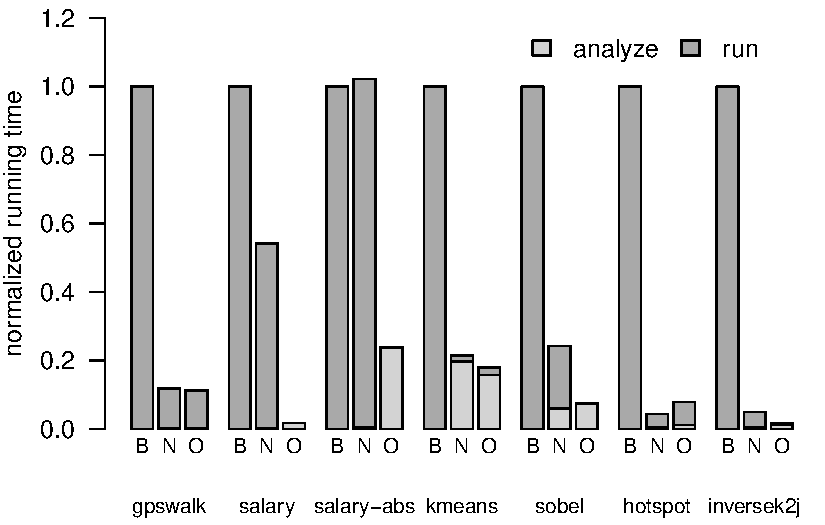
\includegraphics[width=9.5cm]{results/performance}
    \vspace{-1ex}
    \caption{\tool reduces testing time.  We normalize to B: the baseline
      stress-testing technique with 74147 samples. N is \tool without 
      optimizations and O is \tool with optimizations, divided into
      analysis and execution time. Times are averaged over 5 executions.
      We elide error bars as they are very small.}
    \label{passert:fig:performance}
\end{figure}

For most benchmarks, \tool's time is almost exclusively spent on distribution
extraction and optimization, which means optimizations are effective at
producing a very small distribution that can be sampled much more efficiently
than the original program.
The exception is \bench{gpswalk}, where the analysis executed in
\perfdata{time-gpswalk-sample-analyze} seconds
but sampling the resulting distribution took over a minute.
That program's probability distribution consists of thousands of independent
Rayleigh distributions, each with a different parameter as reported by the GPS
sensor, so it cannot take advantage of optimizations that exploit many
samples from identical distributions.

\paragraph{Effect of Optimizations}
We evaluated a variant of \tool with optimizations disabled. This
version simply performs distribution extraction and samples the
resulting distribution.  The middle bars labeled N in
Figure~\ref{passert:fig:performance} show the normalized running time of this
non-optimizing \tool variant.

The effectiveness of the optimizations varies among the benchmarks.
On one extreme, optimizations
reduce the execution time for \bench{salary} from
\perfdata{time-salary-noopt-run} seconds to a fraction of a second.
The unoptimized Bayesian network for \bench{salary-abs} is slightly
\emph{less} efficient than the original program.  The Central Limit
Theorem optimization applies to both and greatly reduces the amount of
sampled computation.  On the other hand, simply evaluating the
extracted distribution delivers a benefit for \bench{gpswalk},
reducing \perfdata{time-gpswalk-dummy-run} to
\perfdata{time-gpswalk-noopt-run} seconds and then optimizations
further reduce this time to just \perfdata{time-gpswalk-sample-run}
seconds.
In a more extreme case, enabling optimizations adds to the analysis time for
\bench{hotspot} but fails to reduce its sampling time.
These programs benefit from eliminating the deterministic
computations involved in timestamp parsing and distance calculation.

\paragraph{Confidence--Performance Trade-off}

Via the confidence and accuracy parameters $\alpha$ and $\epsilon$, \tool
provides rough estimates quickly or more accurate evaluations
using more samples.
% When using fewer samples, the benefits of optimization can be outweighed by
% their costs and the programmer is better off with a brute-force stress-testing
% approach.
To evaluate this trade-off, we lowered the
parameter settings, $\alpha = 0.10$ and $\epsilon = 0.05$, which leads to 2457
samples (about 3\% compared to the more accurate settings above).
Even accounting for analysis time, \tool yields a harmonic mean
\perfdata{o-speedup-harmmean-lowc}
speedup over the baseline in this relaxed configuration.


\section{Discussion}

\sysname differs from the other projects in this dissertation in its focus on a
robust, open-source, end-to-end implementation.
The goal is to demonstrate that a common compiler infrastructure can address
the common concerns for a wide variety of realistic approximation
techniques---in the same way that a classical compiler infrastructure like
LLVM provides all the tools that an intrepid compiler hacker needs to build
new optimizations.
This level of generality required that we solve two common challenges:
balancing programmer insight with automation,
and bridging the gap between fine-grained annotations and coarse-grained
optimizations.

The \sysname source code and documentation is available online at: \\
\url{http://sampa.cs.washington.edu/accept}

